% Funcionamiento de la interfaz inductiva.

\chapter{Acoplamiento Inductivo}
\label{cap:AcoplamientoInductivo}

Para poder avanzar sobre el diseño del circuito integrado primero se debe 
tener una clara idea del comportamiento de la interfaz inductiva. Se debe 
conocer el mecanismo de transferencia de energía entre lector y transponder 
de forma tal de poder asegurar una adecuada alimentación de los circuitos y 
además comprender como se realiza la transmisión de información a través del 
proceso de modulación de carga. En este capítulo se tratarán estos 
temas de forma general y se finalizará con la creación de un modelo de 
SPICE de la interfaz inductiva que luego permitirá realizar simulaciones
de los diseño completo en condiciones reales de trabajo.


\section{Transmisión de la energía}
\label{sec:TransmisionDeLaEnergia}

La interfaz consta de dos inductores, el del lector y el del transponder, 
separados una distancia de algunos centímetros. La transferencia de energía 
se da de forma similar a un transformador, salvo que en este caso el 
coeficiente de acoplamiento es bajo, ya que al no existir un núcleo 
ferromagnético las líneas de campo se encuentran dispersas por el espacio.

En la figura \ref{fig:ModeloAcoplamientoInductivo} se observa un modelo 
simplificado del sistema que sirve para analizar de qué parámetros depende 
la alimentación del transponder. Allí el lector se encuentra modelado como 
una fuente de corriente ideal que alimenta un inductor de inductancia \(
L_{PCD}\). El inductor está acoplado a la antena del transponder, de 
inductancia \(L_{PICC}\), y por lo tanto existe una inductancia mutua \(M\) 
entre ellos. Esta inductancia mutua puede definirse en función de las 
inductancias de las antenas y el coeficiente de acoplamiento \((k)\) como: 
\[M=k \cdot \sqrt{L_{PCD} \cdot L_{PICC}}\]

Se debe notar que todos estos parámetros dependen sólo de la forma y 
disposición de las antenas, lo que se deberá tener en cuenta a la hora de 
hacer los cálculos.

Luego, con el objetivo de mejorar el alcance, se suele utilizar un capacitor 
en paralelo con la antena del transponder, lo que forma un circuito 
resonante LC de elevada \emph{selectividad} (Q). Sin embargo el circuito 
resonante no es imprescindible para el funcionamiento del dispositivo y su 
utilización depende del alcance deseado. Si la tensión inducida en la antena 
a la distancia de trabajo es suficiente entonces el capacitor \(C_{PICC}\) 
puede no utilizarse.

Por último, el circuito integrado en el transponder fue modelado como una 
carga resistiva \(R_{PICC}\), que como primera aproximación es válida ya 
que, cuando el dispositivo tiene que limitar la tensión a través del 
regulador, éste se comporta como una carga resistiva.

\begin{figure}
	\centering
	\shorthandoff{<>}
	\begin{circuitikz}[european voltages] \draw
		(0,0) -- (-2,0) to [sI, l=$I_s$] (-2,2)
		(0,0) to [L, l^=$L_{PCD}$] (0,2) -- (-2,2)
		(2,0) to [L, l_=$L_{PICC}$] (2,2) -- (4.5,2)
		(4.5,0) to [C, l_=$C_{PICC}$] (4.5,2) -- (8,2)
		(8,0) to [R, l_=$R_{PICC}$] (8,2)
		(2,0) -- (5,0) -- (8,0)
		(7.8,0) to [open, v^>=$V_{PICC}$] (7.8,2);
		\draw[dashed, <->, thick] (.1,1.7) .. controls (0.66,2) and (1.32,2) .. (1.9,1.7);
		\draw (1,2.2) node[] {$M$};
	\end{circuitikz}
	\shorthandon{<>}
	\caption{Modelo simplificado del acoplamiento inductivo existente entre lector y transponder.}
	\label{fig:ModeloAcoplamientoInductivo}
\end{figure}

En principio interesa conocer de qué depende la tensión inducida en el 
transponder. Haciendo los cálculos para el circuito funcionando en régimen 
senoidal permanente a una frecuencia \(f = \sfrac{\omega}{2 \pi}\) se 
obtiene:

\begin{equation}
	\label{eq:VpiccGenerico}
	\bar{V}_{PICC} = \frac{j \omega \cdot M \cdot \bar{I}_s \cdot R_{PICC}}{R_{PICC} \left(1-\omega^2 \cdot L_{PICC} \cdot C_{PICC} \right) + j \omega \cdot L_{PICC}}
\end{equation}

El módulo de la tensión inducida puede calcularse para los siguientes casos:

\begin{enumerate}
	\item El circuito tanque LC del transponder puede estar sintonizado a la 
	frecuencia de la portadora transmitida por el lector, cumpliéndose que \(
	\omega^2=\frac{1}{L_{PICC} \cdot C_{PICC}}\), y por lo tanto:
	\begin{equation}
		\label{eq:VpiccRLC}
		V_{PICC} = k \cdot \sqrt{\frac{L_{PCD}}{L_{PICC}}} \cdot R_{PICC} \cdot I_s
	\end{equation}
	
	\item Puede no utilizarse el capacitor en paralelo con \(L_{PICC}\), 
	entonces \(C_{PICC}=0\) y el módulo de la tensión inducida queda:
	\begin{equation}
		\label{eq:VpiccRL}
		V_{PICC} = \omega \cdot k \cdot \frac{\sqrt{L_{PCD} \cdot L_{PICC}}}{\sqrt{R_{PICC}^2 + \left( \omega \cdot L_{PICC} \right)^2}} \cdot R_{PICC} \cdot I_s
	\end{equation}
\end{enumerate}

En el primer caso, la tensión inducida en el transponder es proporcional al 
factor de acoplamiento \((k)\), la corriente que produce el campo magnético 
\((I_s)\), la relación entre las inductancias del lector y del transponder, 
y la carga \((R_{PICC})\); mientras que en el segundo caso el campo también 
depende linealmente del coeficiente de acoplamiento, pero la relación con la 
resistencia de carga \(R_{PICC}\) y las inductancias es más compleja. 

En ambos casos, la corriente \(I_s\) tiene una amplitud constante y la 
frecuencia de trabajo también es constante (\(\omega=\mathrm{cte}\)). 
Además, las inductancias dependen solo de la forma de las antenas y no 
cambian durante la operación del transponder, por lo que también son 
constantes.

Ahora bien, el factor de acoplamiento puede variar dentro de un amplio 
rango, ya que el transponder es acercado y alejado del lector durante el uso 
normal, mientras que la tensión inducida en la antena debe mantenerse por 
encima de la tensión mínima de funcionamiento de los circuitos y por debajo 
de la tensión máxima permitida por el proceso CMOS. Si bien puede acotarse 
el factor de acoplamiento a un rango de funcionamiento deseado, lo que se 
traduce en distancias mínima y máxima de lectura, es conveniente regular la 
tensión inducida en la antena y así evitar superar los límites de tensión. 
Esto se hace variando la resistencia equivalente del transponder \(R_{PICC}\)
de forma tal que cancele la variación de tensión debida a \(k\).

Como se dijo antes, los valores de \(k\), \(L_{PCD}\) y \(L_{PICC}\) 
dependen de variables geométricas como la distancia entre antenas, la forma, 
cantidad de vueltas, etc. La estimación de estos parámetros puede hacerse a 
través de programas de cálculo numérico que resuelven las ecuaciones 
diferenciales asociadas a determinada estructura y para ello se utilizó el 
software \emph{FastHenry} \cite{FastHenry}, que realiza el cálculo de 
resistencia e inductancia de conductores en tres dimensiones a distintas 
frecuencias.

En cuanto a la disposición de las antenas, el arreglo definido en el 
estándar ISO/IEC 10373--6 \cite{ISO10373Part6} fue utilizado como 
referencia. Para la antena del lector (PCD) se utilizó una espira de 
\SI{15}{\centi\meter} de diámetro, según se indica en la norma; y a 
una distancia de \SI{3.75}{\centi\meter} se ubicó la antena del circuito 
integrado, cuyo diseño fue tomado de 
experiencias previas \cite{PosterCASE} y sirvió como 
punto de partida para el análisis de la tensión inducida.

La estructura de antenas fue procesada con el programa \emph{FastHenry} y se 
obtuvo la inductancia de la antena del lector \((L_{PCD})\), el coeficiente 
de acoplamiento \((k)\) y la inductancia de la antena del transponder \(
(L_{PICC})\). Sin embargo, con el propósito de encontrar el valor más 
adecuado para \(L_{PICC}\)  se trazaron los gráficos de la figura \ref
{fig:TensionInducida} en donde se observa la tensión inducida \(V_{PICC}\) 
en función de la carga \(R_{PICC}\) suponiendo que \(L_{PICC}\) varía entre 
\SI{1}{\micro\henry} y \SI{20}{\micro\henry} y manteniendo todos los demás 
parámetros constantes, incluido el coeficiente de acoplamiento. Si bien este 
último se modifica al cambiar la cantidad de vueltas del inductor, de lo 
cuál depende \(L_{PICC}\), en la extracción de parámetros se observó que \(k
\) se mantiene aproximadamente constante si la distancia entre antenas no 
varía. %\todo{Esto se podría mostrar con un gráfico de k en función de L2}

\begin{figure}
	\centering
	\shorthandoff{<>}
	\begin{tikzpicture}
	\matrix {
		\begin{axis}[
				small,
				xmin=0,
				xmax=2000,
				ymin=0,
				ymax=12,
				ylabel={\(V_{PICC} \left[V\right]\)},
				grid=major,
				minor x tick num=1,
				legend style={font=\footnotesize}
			]
			\foreach \l in {1e-6, 5e-6, 10e-6, 15e-6, 20e-6} {
				\addplot[
					domain=1:2000]
					{8.52e7*0.062*sqrt((470e-9)*\l)*x/sqrt(x^2+(8.52e7*\l)^2))*0.456};
			};
			\draw[->, thick] (axis cs:1750,1) .. controls (axis cs:1750,3) and (axis cs:1650,5) .. (axis cs:1500,6) node[anchor=east] {$L_{PICC}\uparrow$};
			\draw (axis cs:300,10) node[fill=white, draw,double,rounded corners] {$H_{\text{mín}}$};
		\end{axis}
		&
		\begin{axis}[
				small,
				xmin=0,
				xmax=2000,
				ymin=0,
				ymax=12,
				grid=major,
				minor x tick num=1,
				legend style={font=\footnotesize}
			]
			\foreach \l in {1e-6, 5e-6, 10e-6, 15e-6, 20e-6} {
				\addplot[
					domain=1:2000]
					{8.52e7*0.062*sqrt((470e-9)*\l)*x/sqrt(x^2+(8.52e7*\l)^2))*1.14};
			};
			\draw[->, thick] (axis cs:1750,1) node [anchor=south east] {$L_{PICC}\uparrow$} .. controls (axis cs:1750,5) and (axis cs:1700,7) .. (axis cs:1500,10);
			\draw (axis cs:300,10) node[fill=white, draw,double,rounded corners] {$H_{\text{máx}}$};
		\end{axis}
		\\
		%
		\begin{axis}[
				small,
				xmin=0,
				xmax=2000,
				ymin=0,
				ymax=12,
				xlabel={\(R_{PICC} \left[ \Omega \right]\)},
				ylabel={\(V_{PICC} \left[V\right]\)},
				grid=major,
				minor x tick num=1,
				legend style={font=\footnotesize}
			]
			\foreach \l in {1e-6, 5e-6, 10e-6, 15e-6, 20e-6} {
				\addplot[
					densely dotted,
					domain=1:2000]
					{0.062*sqrt((470e-9)*\l)*x*0.456/\l};
			};
			\draw[<-, thick] (axis cs:1100,3) node [anchor=north west] {$L_{PICC}\uparrow$} .. controls (axis cs:900,7) and (axis cs:500,8) .. (axis cs:200,9);
			\draw (axis cs:1700,10) node[fill=white, draw,double,rounded corners] {$H_{\text{mín}}$};
		\end{axis}
		&
		\begin{axis}[
				small,
				xmin=0,
				xmax=2000,
				ymin=0,
				ymax=12,
				xlabel={\(R_{PICC} \left[ \Omega \right]\)},
				grid=major,
				minor x tick num=1,
				legend style={font=\footnotesize}
			]
			\foreach \l in {1e-6, 5e-6, 10e-6, 15e-6, 20e-6} {
				\addplot[
					densely dotted,
					domain=1:2000]
					{0.062*sqrt((470e-9)*\l)*x*1.14/\l};
			};
			\draw[<-, thick] (axis cs:750,7) node [anchor=north west] {$L_{PICC}\uparrow$} .. controls (axis cs:600,8) and (axis cs:400,8.3) .. (axis cs:200,8.4);
			\draw (axis cs:1700,10) node[fill=white, draw,double,rounded corners] {$H_{\text{máx}}$};
		\end{axis}
		\\
	};
	\end{tikzpicture}
	\shorthandon{<>}
	\caption{\(V_{PICC}\) en función de \(R_{PICC}\) con \(L_{PICC}\) 
	entre \SI{1}{\micro\henry} y \SI{20}{\micro\henry}. Los gráficos 
	superiores muestran la tensión inducida cuando no se utiliza el 
	capacitor \(C_{PICC}\), mientras que en los inferiores el circuito 
	tanque LC se mantiene sintonizado a la frecuencia de la portadora. 
	\(L_{PCD}=\SI{0.47}{\micro\henry}\); 
	\(I_{s}^{min}=\SI{0.456}{\ampere}\); 
	\(I_{s}^{max}=\SI{1.14}{\ampere}\); 
	\(k=0,062\)}
	\label{fig:TensionInducida}
\end{figure}

Además, para construir los gráficos se calculó  
la corriente \(I_s\) necesaria para obtener las intensidades mínima y máxima 
de campo magnético, dadas en la tabla \ref{tab:NivelesDeCampo}, sobre la 
antena del transponder. Para el cálculo se modeló a la antena del PCD 
como una espira de \SI{15}{\centi\meter} de diámetro y utilizando la 
ley de \emph{Biot--Savart} se obtuvo la expresión del campo a lo largo 
de su eje. Luego, igualando esta expresión a los niveles de campo 
mínimo y máximo se obtuvieron las corrientes necesarias para producirlos.

En la figura \ref{fig:TensionInducida} se observa que en el caso en que no 
se utiliza el capacitor \(C_{PICC}\), la tensión inducida en la antena del 
transponder tiende a \(\omega M I_s\) cuando la resistencia \(R_{PICC}\) 
tiende a infinito; mientras que con el circuito tanque LC la tensión tiende 
idealmente a infinito si se lo deja sin carga. Además, suponiendo que el 
circuito integrado equivale a una carga nominal de \SI{2}{\kilo\ohm}, a la 
distancia de \SI{3.75}{cm} \(V_{PICC}\) es más que suficiente para alimentar 
el dispositivo con el campo mínimo y se excede en varios volts cuando la 
intensidad del campo es máxima.

Por otro lado, el uso del capacitor \(C_{PICC}\), si bien tiene la ventaja 
de incrementar la selectividad del circuito y por lo tanto aumentar la 
tensión inducida, también tiene el inconveniente de que se restringe el 
ancho de banda para la transmisión de datos. Como se vio en la sección \ref
{sec:ISO14443_2}, la transmisión de datos por modulación de carga se realiza 
utilizando una sub-portadora de \SI{847,5}{\kilo\hertz}, y por lo tanto el 
espectro en frecuencia contiene la señal portadora de \SI{13.56}{\mega\hertz
} y dos bandas laterales separadas a \SI{847,5}{\kilo\hertz} de la 
portadora, como se observa en la figura \ref{fig:EspectroModulacionCarga}. 
Entonces el ancho de banda del canal debe ser de por lo menos \SI{1.7}{
\mega\hertz} para atenuar las bandas laterales \SI{3}{\decibel} como máximo. 
El ancho de banda del circuito RLC está relacionado con el factor de 
selectividad de la siguiente forma:
\[ Q = \frac{f_c}{\Delta f} \leq \frac{\SI{13.56}{\mega\hertz}}{\SI{1.7}{\mega\hertz}} \approx 8
\]

\begin{figure}
	\centering
	\shorthandoff{<>}
	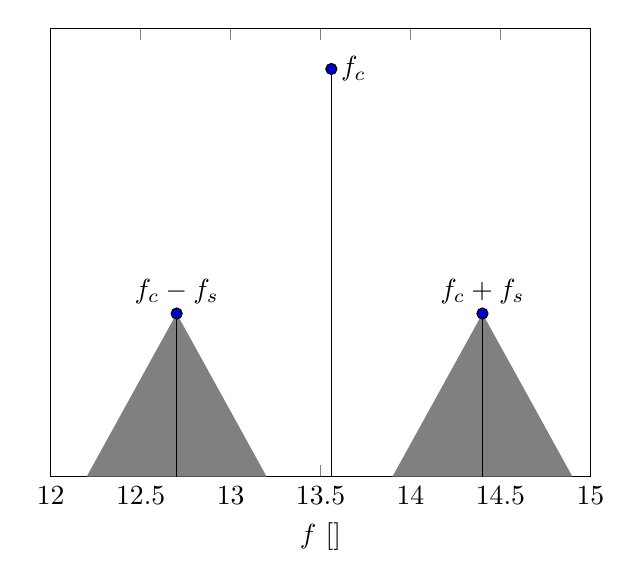
\begin{tikzpicture}
		\begin{axis}[
			ytick=\empty,
			ymin=0,
			xmin=12,
			xmax=15,
			xlabel={\(f\) [\si{\mega\hertz}]}
			]
			\fill[gray] (axis cs:12.7,40) -- (axis cs:12.2,0) -- (axis cs:13.2,0) -- (axis cs:12.7,40);
			\fill[gray] (axis cs:14.4,40) -- (axis cs:13.9,0) -- (axis cs:14.9,0) -- (axis cs:14.4,40);
			\addplot+[ycomb, black] plot coordinates
				{(13.56,100) (12.7,40) (14.4,40)};
			\draw (axis cs:13.56,100) node[fill=white, anchor=west] {$f_c$};
			\draw (axis cs:12.7,40) node[fill=white, anchor=south] {$f_c-f_s$};
			\draw (axis cs:14.4,40) node[fill=white, anchor=south] {$f_c+f_s$};
		\end{axis}
	\end{tikzpicture}
	\shorthandon{<>}
	\caption{Espectro de la señal cuando es modulada con la sub-portadora para enviar datos desde la PICC hacia el PCD.}
	\label{fig:EspectroModulacionCarga}
\end{figure}

Además, se debe cumplir la condición de resonancia del circuito RLC 
paralelo, es decir \(\omega_0 = \sfrac{1}{\sqrt{L_{PICC} C_{PICC}}}\), y con 
esta condición el \(Q\) del circuito queda:
\[ Q = \frac{R_{PICC}}{\omega_0 L_{PICC}} \]

En la figura \ref{fig:QvsL_CvsL} se graficó el factor Q en función de \(
L_{PICC}\) suponiendo una carga de \SI{2}{\kilo\ohm}, y \(C_{PICC}\) en 
función de \(L_{PICC}\) utilizando la condición de resonancia del circuito 
RLC paralelo.

\begin{figure}
	\centering
	\shorthandoff{<>}
	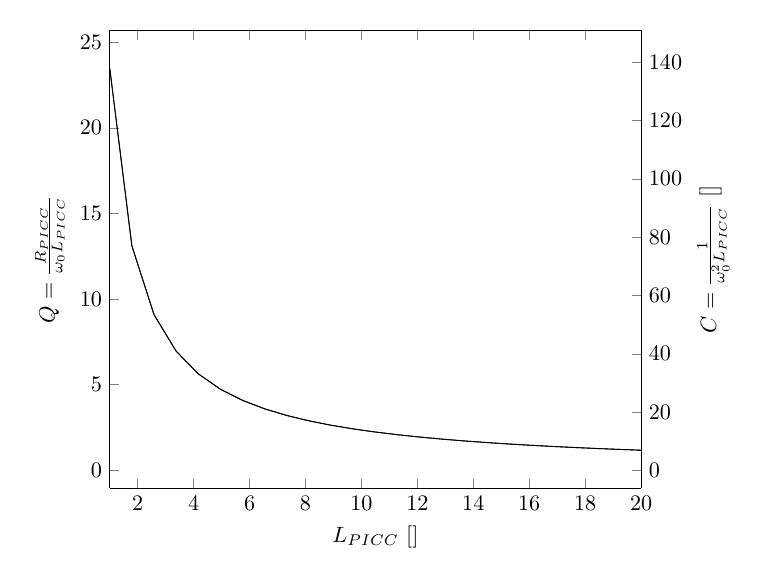
\begin{tikzpicture}[scale=0.8]
		% let both axes use the same layers
		%\pgfplotsset{set layers}
		\begin{axis}[
			scale only axis,
			xmin=1,xmax=20,
			domain=1:20,
			axis y line*=left,% the ’*’ avoids arrow heads
			xlabel={\(L_{PICC}\) [\si{\micro\henry}]},
			ylabel={\(Q = \frac{R_{PICC}}{\omega_0 L_{PICC}}\)}]
			\addplot[black]{2000/((8.52e7)*(x*1e-6))};
		\end{axis}

		\begin{axis}[
			scale only axis,
			xmin=1,xmax=20,
			domain=1:20,
			axis y line*=right,
			axis x line=none,
			ylabel={\(C=\frac{1}{\omega_0^2 L_{PICC}}\) [\si{\pico\farad}]}]
			\addplot[black] {1e12/(7.25e15*(x*1e-6)};
		\end{axis}
	\end{tikzpicture}
	\shorthandon{<>}
	\caption{Factor Q y capacidad de \(C_{PICC}\) en función de \(L_{PICC}\), cumpliendo la condición de resonancia.}
	\label{fig:QvsL_CvsL}
\end{figure}

El análisis realizado hasta el momento da una idea de la inductancia, 
capacidad y carga que pueden ser utilizadas para obtener una tensión 
suficiente como para alimentar el circuito integrado. Sin embargo también es 
muy importante saber de qué forma realizar la modulación de carga para 
cumplir con la amplitud de modulación dada por el estándar. A continuación 
se analizará la estructura de antenas dada por la norma ISO/IEC 10373--6, 
que es utilizada para medir dicha amplitud, y luego utilizando la 
herramienta \emph{FastHenry} se realizará un modelo de la estructura para 
luego realizar simulaciones con SPICE.

\section{Transmisión por modulación de carga}
\label{sec:InterfIndTransDatos}

Para transmitir información el transponder aumenta y disminuye su consumo, 
lo que se traduce en una variación de amplitud en la antena del lector, que 
es detectada por este y traducida a bit de datos. El aumento y disminución 
del consumo se realiza conectando y desconectando una carga dentro del 
transponder que puede ser de tipo resistiva o capacitiva. El estándar 
ISO/IEC 14443 define un valor mínimo para la amplitud de modulación de carga 
(figura \ref{fig:AmplitudesPICC_PCD}) y también determina de que forma se 
debe realizar la medición de ese parámetro. Para ello se debe utilizar el 
arreglo de antenas definido por la norma ISO/IEC 10373--6 \cite
{ISO10373Part6}, que se observa en la figura \ref{fig:ArregloDeAntenas}. El 
mismo consta de una antena transmisora de \SI{15}{\centi\meter} de diámetro, 
que emite la señal portadora de \SI{13.56}{\mega\hertz}, con dos antenas más 
pequeñas, una delante y la otra detrás, que son utilizadas para medir la 
amplitud de la modulación de la PICC. Los tres inductores deben fabricarse 
sobre placas de circuito impreso tipo FR--4 de \SI{170}{\milli\meter} de 
lado y las antenas \(L_A\) y \(L_B\) son conectadas de forma tal que la suma 
de las tensiones inducidas debidas a la portadora se anulan. Finalmente, el 
\emph{Device Under Test} (DUT), que aquí es el transponder, se coloca del 
lado opuesto al cobre de uno de los PCBs de medición.

\begin{figure}
	\centering
	\includegraphics{ArregloDeAntenas}
	\caption{Arreglo de antenas definido por el estándar ISO/IEC 10373--6. 
		Dimensiones en milímetros.}
	\label{fig:ArregloDeAntenas}
\end{figure}

En la figura \ref{fig:ModeloDelArregloParaModulacionDeCarga} se observa el 
circuito equivalente del arreglo. Los inductores \(L_A\) y \(L_B\) se 
conectan en serie con un resistor variable con punto medio y desde este nodo 
se mide la amplitud de la modulación mediante un osciloscopio. El 
resistor variable se ajusta de forma tal de llevar a 
cero la tensión \(V_{sens}\) y por lo tanto eliminar posibles desbalances en 
la estructura. En este caso se supuso que la estructura está
perfectamente balanceada y por lo tanto los resistores son iguales.

\begin{figure}
	\centering
	\shorthandoff{<>}
	\resizebox{\textwidth}{!}{
		\begin{circuitikz}[european voltages] \draw
			(1,0) to [short, o-] (0,0) 
			to [L, l_=$L_{PCD}$] (0,2) 
			to [short, i<=$i_{PCD}$, -o] (1,2)
			(-0.2,0) to [open, v^>=$V_{PCD}$] (-0.2,2)
			(0,2) node[below right=2mm] {$\bullet$}
			
			(4,0) node[ground]{} to [L, l=$L_{B}$, o-o] (4,2)
			to [short, i^<=$i_{sens}$] (4,4)
			to [R, l=$R_{sens}$, -*] (0,4) to [R, l=$R_{sens}$] (-4,4)
			to [short, i<^=$i_{sens}$] (-4,2)
			to [L, l=$L_{A}$, o-o] (-4,0) node[ground]{}
			(4.2,0) to[open, v<=$V_{B}$] (4.2,2)
			(-4.2,2) to[open, v<=$V_{A}$] (-4.2,0)
			(0,4) to [short, -o] (0,4.5) node[above]{$V_{sens}$}
			(4,0) node[above left=2mm] {$\bullet$}
			(-4,2) node[below right=2mm] {$\bullet$}
			
			(-6,0) to [L, l=$L_{PICC}$, o-o] (-6,2)
			to [short, i=$i_{PICC}$] (-8,2) 
			to [generic] (-8,0) -- (-6,0)
			(-8.3,2) to [open, v<=$V_{PICC}$] (-8.3,0)
			(-6,2) node[below right=2mm] {$\bullet$};
		\end{circuitikz}
	}	
	\shorthandon{<>}
	\caption{Conexionado del arreglo de antenas de la figura \ref{fig:ArregloDeAntenas}.}
	\label{fig:ModeloDelArregloParaModulacionDeCarga}
\end{figure}

Haciendo los cálculos se llega a que la 
amplitud de la tensión medida por el osciloscopio cumple con la siguiente 
ecuación:

\begin{equation}
	\label{eq:Vsens}
	V_{sens} = 0.45 \cdot \omega \cdot M_{A\text{-}PICC} \cdot i_{PICC}
\end{equation}

\(M_{A\text{-}PICC}\) depende del factor de acoplamiento y por lo tanto de 
la distancia entre el transponder y la antena \(L_A\), que en el caso del 
arreglo de la norma es constante. Entonces basta variar \(i_{PICC}\) para 
lograr una variación en la amplitud de \(V_{sens}\) y es esta variación en 
la amplitud de \(V_{sens}\) lo que el estándar define como amplitud de 
modulación.

La corriente \(i_{PICC}\) puede calcularse de la siguiente forma:

\begin{equation}
	i_{PICC} = \left|\frac{\bar{V}_{PICC}}{\bar{Z}_{PICC}}\right|
\end{equation}

Para mantener la generalidad se supone que se tiene un circuito RLC en el 
transponder y entonces \(\bar{V}_{PICC}\) cumple con la expresión de la 
ecuación \eqref{eq:VpiccGenerico} y \(\bar{Z}_{PICC}\) es la impedancia de 
un circuito RC paralelo. Teniendo esto en cuenta, la expresión de \(i_{PICC}
\) queda:

\begin{equation}
	i_{PICC} = \frac{\sqrt{\left(\omega^2 M_{\text{pcd-picc}} R_{PICC} 
	C_{PICC}\right)^2 + \left(\omega M_{\text{pcd-picc}}\right)^2}}{\sqrt{\left(R_{PICC}-\omega^2 R_{PICC} L_{PICC} C_{PICC}\right)^2 + \left(\omega L_{PICC}\right)^2}} \cdot I_{PCD}
\end{equation}

Como se dijo al principio, existen dos tipos de modulación de carga, 
resistiva y capacitiva, en las que cambia el tipo de componente utilizado 
para la modulación. Además, como se mostró en la sección previa, para 
alimentar el circuito integrado existe la posibilidad de utilizar el 
circuito tanque LC en resonancia o solo el inductor conectado directamente 
al chip. Por lo tanto la modulación de carga puede consistir en 
agregar/quitar un capacitor en paralelo con el del tanque LC, de forma tal 
de variar la capacidad total del circuito tanque; o bien agregar/quitar una 
carga resistiva, en cuyo caso puede utilizarse o no el capacitor \(C_{PICC}\)
. En la figura \ref{fig:PlotsModulacionDeCarga} se trazaron los gráficos 
correspondientes a la ecuación \eqref{eq:Vsens} en los tres casos posibles y 
suponiendo que el tag tiene aplicado el campo mínimo ---es decir, se calculó 
\(I_{PCD}\) para que en la ubicación del transponder la amplitud del campo 
sea mínima---. En estas condiciones la amplitud de la modulación de carga 
debe ser de \SI{18}{\milli\volt} como mínimo según el gráfico de la figura 
\ref{fig:AmplitudesPICC_PCD}.

\begin{figure}
	\centering
	\begin{subfigure}{0.45\textwidth}
		\centering
		\shorthandoff{<>}
		\resizebox{\textwidth}{!}{
			\begin{tikzpicture}
				% let both axes use the same layers
				%\pgfplotsset{set layers}
				\def\w{8.52e7}
				\def\mpcdpicc{120e-9}
				\def\mapicc{343e-9}
				\def\cpicc{17.22e-12}
				\def\lpicc{8e-6}
				\def\ipcd{0.456}
				\begin{axis}[
					small,
					domain=0.1:3,
					grid=major,
					minor x tick num=1,
					ymin=0,
					ymax=0.4,
					xlabel={\(R_{PICC}\) [\si{\kilo\ohm}]},
					ylabel={\(V_{sens}\) [\si{\volt}]},
					legend pos={north west}]
					%\addplot[black]{\ipcd*0.45*\w*\mapicc*sqrt((\w^2*\mpcdpicc*\cpicc*x*1000)^2+(\w*\mpcdpicc)^2)/sqrt((x*1000-\w^2*x*1000*\lpicc*\cpicc)^2+(\w*\lpicc)^2)};
					\addplot[black] table[x index=0,y index=1] {plots/VsensVsRpicc_RLC.dat};
					\addlegendentry{RLC \(\left(\omega^2=\frac{1}{LC}\right)\)}
				
					\def\cpicc{0}
					%\addplot[dashed]{\ipcd*0.45*\w*\mapicc*sqrt((\w^2*\mpcdpicc*\cpicc*x)^2+(\w*\mpcdpicc)^2)/sqrt((x-\w^2*x*\lpicc*\cpicc)^2+(\w*\lpicc)^2)};
					\addplot[dashed] table[x index=0,y index=1] {plots/VsensVsRpicc_RL.dat};
					\addlegendentry{RL}
				\end{axis}
			\end{tikzpicture}
		}
		\shorthandon{<>}
		\caption{Modulación de carga resistiva. \(L_{PICC}=\SI{8}{\micro\henry}; C_{PICC}=\SI{17.2}{\pico\farad};\\ H=H_{\text{mín}}\)}
		\label{fig:VsensModulacionR}
    \end{subfigure}%
    \quad
    \begin{subfigure}{0.45\textwidth}
	    \centering
		\shorthandoff{<>}
		\resizebox{\textwidth}{!}{
			\begin{tikzpicture}
				\def\w{8.52e7}
				\def\mpcdpicc{120e-9}
				\def\mapicc{343e-9}
				\def\rpicc{2000}
				\def\lpicc{8e-6}
				\def\ipcd{0.456}
				\begin{axis}[
					small,
					domain=0:22,
					grid=major,
					minor x tick num=1,
					ymin=0,
					ymax=0.4,
					xlabel={\(C_{PICC}\) [\si{\pico\farad}]},
					ylabel={\(V_{sens}\) [\si{\volt}]},
					legend pos={north west}]
					%\addplot[black]{\ipcd*0.45*\w*\mapicc*sqrt((\w^2*\mpcdpicc*x*1e-12*\rpicc)^2+(\w*\mpcdpicc)^2)/sqrt((\rpicc-\w^2*x*1e-12*\lpicc*\rpicc)^2+(\w*\lpicc)^2)};
					\addplot[black] table[x index=0,y index=1] {plots/VsensVsCpicc_RLC.dat};
					\addlegendentry{RLC}
				\end{axis}
			\end{tikzpicture}
		}
		\shorthandon{<>}
		\caption{Modulación de carga capacitiva. \(L_{PICC}=\SI{8}{\micro\henry}; R_{PICC}=\SI{2}{\kilo\ohm};\\ H=H_{\text{mín}}\)}
		\label{fig:VsensModulacionC}
    \end{subfigure}%
    \caption{Tensión \(V_{sens}\) medida a la salida del arreglo de la 
		figura \ref{fig:ArregloDeAntenas} para los distintos tipos de modulación 
		de carga posibles.}
	\label{fig:PlotsModulacionDeCarga}
\end{figure}

En la figura \ref{fig:VsensModulacionR} se observa \(V_{sens}\) en función 
de la resistencia de carga, cuando se utiliza un circuito RLC sintonizado a 
la frecuencia de resonancia y cuando se utiliza sólo un circuito RL. En el 
primero caso, si la carga nominal del circuito integrado del transponder es 
de \SI{2}{\kilo\ohm}, basta con conectar una pequeña carga en paralelo para 
lograr una amplitud de modulación importante, mientras que en el caso del 
circuito RL, la variación de la resistencia casi no produce variación en la 
amplitud de \(V_{sens}\).

Por otro lado, en la figura \ref{fig:VsensModulacionC} se trazó la gráfica 
de \(V_{sens}\) en función de \(C_{PICC}\). En este caso se utiliza un 
circuito RLC cuya frecuencia de resonancia cambia a medida que cambia la 
capacidad de \(C_{PICC}\), lo que logra una gran amplitud de modulación. Del 
gráfico surgen varias posibilidades con respecto a cómo realizar la 
modulación. La primer posibilidad sería comenzar con \(C_{PICC}=0\) y 
conectar una pequeña capacidad interna al circuito integrado de 
aproximadamente \SI{5}{\pico\farad}, haciendo variar \(V_{sens}\) en poco 
más de \SI{20}{\milli\volt}. Otra posibilidad sería utilizar un valor para \(
C_{PICC}\) intermedio entre \SI{0}{\pico\farad} y el valor que hace resonar 
el circuito LC, donde la curva tiene mayor pendiente. De esta forma con una 
capacidad mínima se logra una gran variación en \(V_{sens}\). Y por último 
existe también la posibilidad de utilizar el valor de \(C_{PICC}\) que hace 
resonar al tanque LC y agregando o quitando capacidad lograr la amplitud de 
modulación deseada. 

\section{Modelo de SPICE del arreglo de antenas}
\label{sec:ModeloSpiceAntenas}

Para corroborar las expresiones obtenidas de la tensión inducida en la 
antena de la PICC y la amplitud de la modulación de carga, se construyó un 
modelo de SPICE del arreglo de antenas de la figura \ref
{fig:ArregloDeAntenas}. Gracias a ello, se contó con la posibilidad de 
realizar simulaciones y comparar los resultados obtenidos por ambos métodos.

En la figura \ref{fig:ModeloSpiceArregloAntenas} se muestra el componente de 
\emph{LTSpice} \cite{LTSpice} que contiene el modelo. Se modelaron los 
cuatro inductores del arreglo, \(L_{PCD}\), \(L_{A}\), \(L_{B}\) y \(L_{PICC}
\), donde cada uno fue definido como una inductancia en serie con una 
resistencia equivalente a la frecuencia de trabajo. Los inductores se 
encuentran vinculados mediante coeficientes de acoplamiento que representan 
la influencia de unos sobre otros.

Los parámetros del modelo ---inductancias, resistencias y coeficientes de 
acoplamiento--- fueron obtenidos utilizando el programa de extracción de 
inductancias \emph{FastHenry} \cite{FastHenry}, lo que permitió obtener una 
fiel representación de la realidad. La descripción de la estructura de 
antenas en el formato de \emph{FastHenry} no es trivial, ya que se debe 
crear una lista de nodos y segmentos asignándole a cada uno sus 
coordenadas en el espacio 
a fin de formar la estructura deseada. Para hacer este trabajo más simple y 
dinámico, se elaboró un script de \emph{Octave} \cite{Octave} que 
genera el archivo de entrada para \emph{FastHenry} 
de forma automática. Las antenas fueron parametrizadas en el script de forma 
tal que cambiando solo algunas variables se pueden modificar las dimensiones 
de los inductores, cantidad de vueltas, distancia entre ellas, etc. Una 
vista en tres dimensiones del conjunto de inductores generado puede verse en 
la figura \ref{fig:ArregloDeAntenasVista3D}.

\begin{figure}
	\centering
	\begin{subfigure}{0.45\textwidth}
		\centering
		\includegraphics[width=0.8\textwidth]{ArregloAntenasComponenteLTSpice}
		\caption{Componente que contiene el modelo de SPICE.}
		\label{fig:ModeloSpiceArregloAntenas}
	\end{subfigure}%
	\begin{subfigure}{0.45\textwidth}
		\centering
		\includegraphics[width=0.6\textwidth]{ArregloDeAntenasVista3D}
		\caption{Vista 3D.}
		\label{fig:ArregloDeAntenasVista3D}
	\end{subfigure}%
	\caption{Componente utilizado en \emph{LTSpice} y vista en tres 
		dimensiones del conjunto de inductores ingresado a \emph{FastHenry}.}
	\label{fig:ModeloSpice}
\end{figure}

La antena generada para el transponder es un inductor en forma de espiral 
del tamaño de una tarjeta ID--1 \cite{ISO7810}. Las dimensiones, separación 
entre pistas, ancho de pista, posición y cantidad de vueltas de esta antena 
pueden cambiarse fácilmente modificando los respectivos parámetros en el 
script de \emph{Octave}. 

La salida del programa \emph{FastHenry} es un archivo de texto que contiene 
matrices con las impedancias de cada elemento, las inductancias y los 
coeficientes de acoplamiento, todo esto calculado a la frecuencia 
seleccionada. La elaboración de la \emph{netlist} de SPICE también fue 
automatizada mediante un script de \emph{Octave}, que toma los valores de 
las matrices de salida de \emph{FastHenry} y finalmente escribe el modelo de 
SPICE en un archivo listo para usar junto con el componente de la figura \ref
{fig:ModeloSpiceArregloAntenas}.

Los pasos para la elaboración de la netlist de SPICE se esquematizaron en la 
figura \ref{fig:PasosElaboracionSpice}. El alto nivel de automatización 
permitió llevar la estructura física de las antenas dentro del software \emph
{LTSpice} y por lo tanto observar rápidamente como se reflejan los cambios 
físicos en la respuesta de los circuitos. Además, permitió comparar 
rápidamente los resultados de las simulaciones con los resultados 
obtenidos en la sección precedente.

\begin{figure}
	\centering
	\includegraphics[width=\textwidth]{PasosElaboracionSpice}
	\caption{Proceso de generación de la \emph{netlist} de SPICE.}
	\label{fig:PasosElaboracionSpice}
\end{figure}


\section{Resultados del análisis}

En los análisis realizados en las secciones de transmisión de energía 
y de transmisión de datos por modulación de carga se mostró que 
existen numerosas posibilidades en cuanto al conexionado del circuito 
de antena. Para la transmisión de energía y a partir del modelo simple 
desarrollado, se observó que se tienen dos posibilidades: conectar la 
antena directamente a la entrada del CI, o utilizar un circuito tanque 
LC que mejora la recepción de energía, pero que también limita el 
ancho de banda para la transmisión de datos. Además se observó que 
la amplitud de la tensión generada en la antena es más que suficiente 
para alimentar el dispositivo y en todo caso se debe limitar esa 
amplitud para no dañarlo. 

Una forma efectiva de limitar la tensión inducida en la antena es 
aumentar la carga conectada a ella, según se desprende de la figura 
\ref{fig:TensionInducida}. El consumo nominal del chip, esto es, el 
consumo cuando el regulador/limitador no actúa, se estima será de 
aproximadamente \SI{1}{\milli\ampere}, lo que equivale a una carga 
resistiva de \SI{3}{\kilo\ohm}, suponiendo \SI{3}{\volt} de tensión 
de alimentación. En la figura puede verse como la amplitud de la 
tensión inducida con el circuito tanque LC a carga nominal es mucho 
mayor a los \SI{5}{\volt} necesarios, lo que haría que el 
regulador/limitador de tensión actúe de forma continua para cualquier 
nivel de campo. Por otro lado, con la antena conectada directamente 
al transponder, la tensión inducida alcanza un máximo dado por el 
coeficiente de acoplamiento y la inductancia de las antenas. 
Suponiendo un coeficiente de acoplamiento aproximadamente constante, se 
puede elegir el valor de \(L_{PICC}\) tal que con el campo mínimo 
\(H_{\text{mín}}\) y a carga nominal, se obtenga una tensión de 
\SI{5}{\volt} en la antena. Haciendo esto, el valor de inductancia que 
hizo que se cumplan esas condiciones fue de \SI{8}{\micro\henry}. Con 
este valor, a campo máximo la tensión inducida en la antena alcanzará 
una amplitud de aproximadamente \SI{12}{\volt} y en esta situación el 
regulador/limitador de tensión actuará aumentando la carga vista por 
la antena.

\bigskip
En la sección de transmisión por modulación de carga se analizó el 
arreglo de antenas definido por el estándar para medir la amplitud de 
la modulación y se mostró como variando una carga resistiva o una 
capacitiva se obtiene una variación en la amplitud de la tensión 
medida a la salida del arreglo. Para la transmisión de energía se 
decidió utilizar la antena sin capacidad en paralelo y, como la 
amplitud de \(V_{sens}\) varía muy poco con una carga resistiva 
(figura \ref{fig:VsensModulacionR}), se 
decidió utilizar una modulación capacitiva. De la figura 
\ref{fig:VsensModulacionC} se obtuvo que con una capacidad de 
\SI{8}{\pico\farad}, un valor razonable para integrar dentro de un 
chip, la amplitud de la modulación producida debería ser suficiente para 
cumplir con los requisitos del estándar.

Resumiendo, para la interfaz inductiva se decidió utilizar una antena 
de \SI{8}{\micro\henry} sin capacidad en paralelo, cuyo diseño se puede 
ver en la figura \ref{fig:DisenioAntena}. Se decidió regular la 
tensión inducida variando una carga resistiva dentro del bloque 
regulador/limitador de tensión y por último, para la modulación de 
carga, se decidió utilizar una carga capacitiva también dentro del 
chip.

\begin{figure}
	\centering
	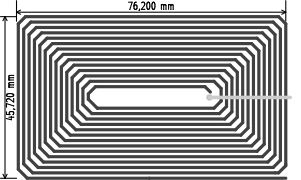
\includegraphics[width=0.6\textwidth]{placa_tag-brd}
	\caption{Antena del transponder fabricada sobre una placa de 
	circuito impreso. Su tamaño es el de una tarjeta ID--1 y su 
	inductancia \SI{8}{\micro\henry}.}
	\label{fig:DisenioAntena}
\end{figure}

% En la tabla \ref{tab:ParametrosAntena} se muestran, a modo de ejemplo, 
% los valores obtenidos luego de realizada la extracción de parámetros 
% del arreglo de antenas del la figura \ref{fig:ArregloDeAntenas} 
% utilizando como DUT el diseño de la figura 
% \ref{fig:DisenioAntena}.
% 
% \begin{table}
	% \centering
	% \begin{tabu}{lcl|lcl}
		% \toprule
		% Parámetro & Valor & Unidad & Parámetro & Valor & Unidad \\  
		% \midrule
		% \(L_{PICC}\)     & \SI{8.11}{}      & \si{\micro\henry} & \(k_{PICC,PCD}\) & \SI{0.062}{}     & -- \\
		% \(R_{PICC}\)     & \SI{1.51}{}      & \si{\ohm}         & \(k_{PICC,LA}\)  & \SI{0.198}{}     & -- \\
		% \(L_{PCD}\)      & \SI{0.47}{}      & \si{\micro\henry} & \(k_{PICC,LB}\)  & \SI{-0.019}{}    & -- \\
		% \(R_{PCD}\)      & \SI{0.167}{}     & \si{\ohm}         & \(k_{PCD,LA}\)   & \SI{0.092}{}     & -- \\
		% \(L_{A}\)        & \SI{0.368}{}     & \si{\micro\henry} & \(k_{PCD,LB}\)   & \SI{-0.092}{}    & -- \\
		% \(R_{A}\)        & \SI{0.388}{}     & \si{\ohm}         & \(k_{LA,LB}\)    & \SI{-0.026}{}    & -- \\
		% \(L_{B}\)        & \SI{0.368}{}     & \si{\micro\henry} &  \\
		% \(R_{B}\)        & \SI{0.388}{}     & \si{\ohm}         &  \\
		% \bottomrule
	% \end{tabu}
	% \caption{Parámetros extraídos mediante \emph{FastHenry} de la 
	% estructura de antenas de la figura \ref{fig:ArregloDeAntenas}.}
	% \label{tab:ParametrosAntena}
% \end{table}
